\documentclass[conference]{IEEEtran}

\usepackage{graphicx}
\usepackage[super]{nth}
\usepackage{xfrac}

\begin{document}
	
	\title{Chinese Borders}
	
	\author{\IEEEauthorblockN{Ida Hönigmann}
		\IEEEauthorblockA{Technical Secondary College\\
			Department of Computer Science\\
			2700 Wiener Neustadt, Austria\\
			Email: hoenigmann.ida@student.htlwrn.ac.at}
	}
	
	\maketitle
	
	\begin{abstract}
		This paper explored the history and current status of the borders China shares with its neighboring countries. To fully understand the current situation the relations between the countries is portrayed. Interesting facts, such as the historic importance of border crossings, the way the population has been influenced by the border and how the borders came to be are explored. Besides an analysis of all land borders a section about the South China Sea focuses on the disputed regions in the ocean.
	\end{abstract}
	\section{Introduction}
	As China is not particularly friendly to most of its neighboring countries and has the longest land border in the world, it is no wonder that there are several disputes and even more interesting facts about these lines on the map.
	
	The topic of Chinese borders gives an insight into Chinese history, for which the Russian and Mongolian relations to China as well as Hong Kong and Macau are examples. It explores who and what gets transported out and into the country, such as workers building the Belt and Road Initiative, products being sold by China and North Koreans fleeing their country. Border disputes and the people living in these regions are yet another interesting case study along the Chinese border to Pakistan, India, Bhutan, Myanmar and Nepal. While one would think being a communist lead country would help increase the relation to China Vietnam and Laos show that China is more picky and looks for more than just general political beliefs. After having established all these interesting relations to all of its bordering countries China on land it tried extending its influence on the South China Sea. 
	
	\section{North Korea}
	Along the border separating China from North Korea lies one of the holy sights of all Koreans: Mount Paektu. \cite{theIndianExpress_explainedWhatIsTheSignificanceOfMtPeaktuForKinJongUn} Here South Koreans as well as North Koreans visit the Heaven Lake, although separated by multiple meters, as to not be able to see one another. From this mountain the two rivers Yalu and Tumen form. These rivers serve as the separation between the two countries.
	
	Further west in Dandong a significant portion of North Korea's trade with the outside world is being moved by trucks over a single bridge. These trucks are being loaded up in China and send to North Korea, where they are unloaded and send back - mostly empty. The imports from China make up about 57\%\cite{wp_economyOfNorthKorea} of Norths Korea's imports in total.
	
	One of the reasons China is exporting so many goods to North Korea is fear of the regime collapse, which would send thousands of North Korean emigrants over the border to China.
	
	As there are already some defectors crossing the border further east, the shallow river is protected by Chinese guards.\cite{yp_anInconvenientBorderWhereChinaMeetsNorthKoreaABCNews} All fleeing persons found, are send back to North Korea, where they will most likely face death.
	
	\section{India, Pakistan and Nepal}
	The border shared with India, Pakistan and Nepal is crowded with border disputes. The rough terrain made it impossible to establish borders for the longest time in history. Now, with the technology to reach these isolated sections, many nations claim their chunk.
	
	\subsection{Jammu and Kashmir}
	When Britain left India, they decided to split the country into a Moslem (now called Pakistan and Bangladesh) and a Hindu (still called India) part, according to the affiliation of people living in each region. In some regions the local ruler could choose to which side the region should belong. In Jammu and Kashmir, the ruler opted for independence of both, but after being invaded by Pakistan, turned to India.
	
	The northern part of Jammu and Kashmir, Aksai Chin, is hard to access from India. So, when China built a road through this terrain during the 1950s, India did not notice until 1957. Since then Aksai Chin in administered by China. A section of the road can be seen in figure~\ref{pic:india_jammuAndKashmir_road}.
	
	\begin{figure}[t]
	\centering
	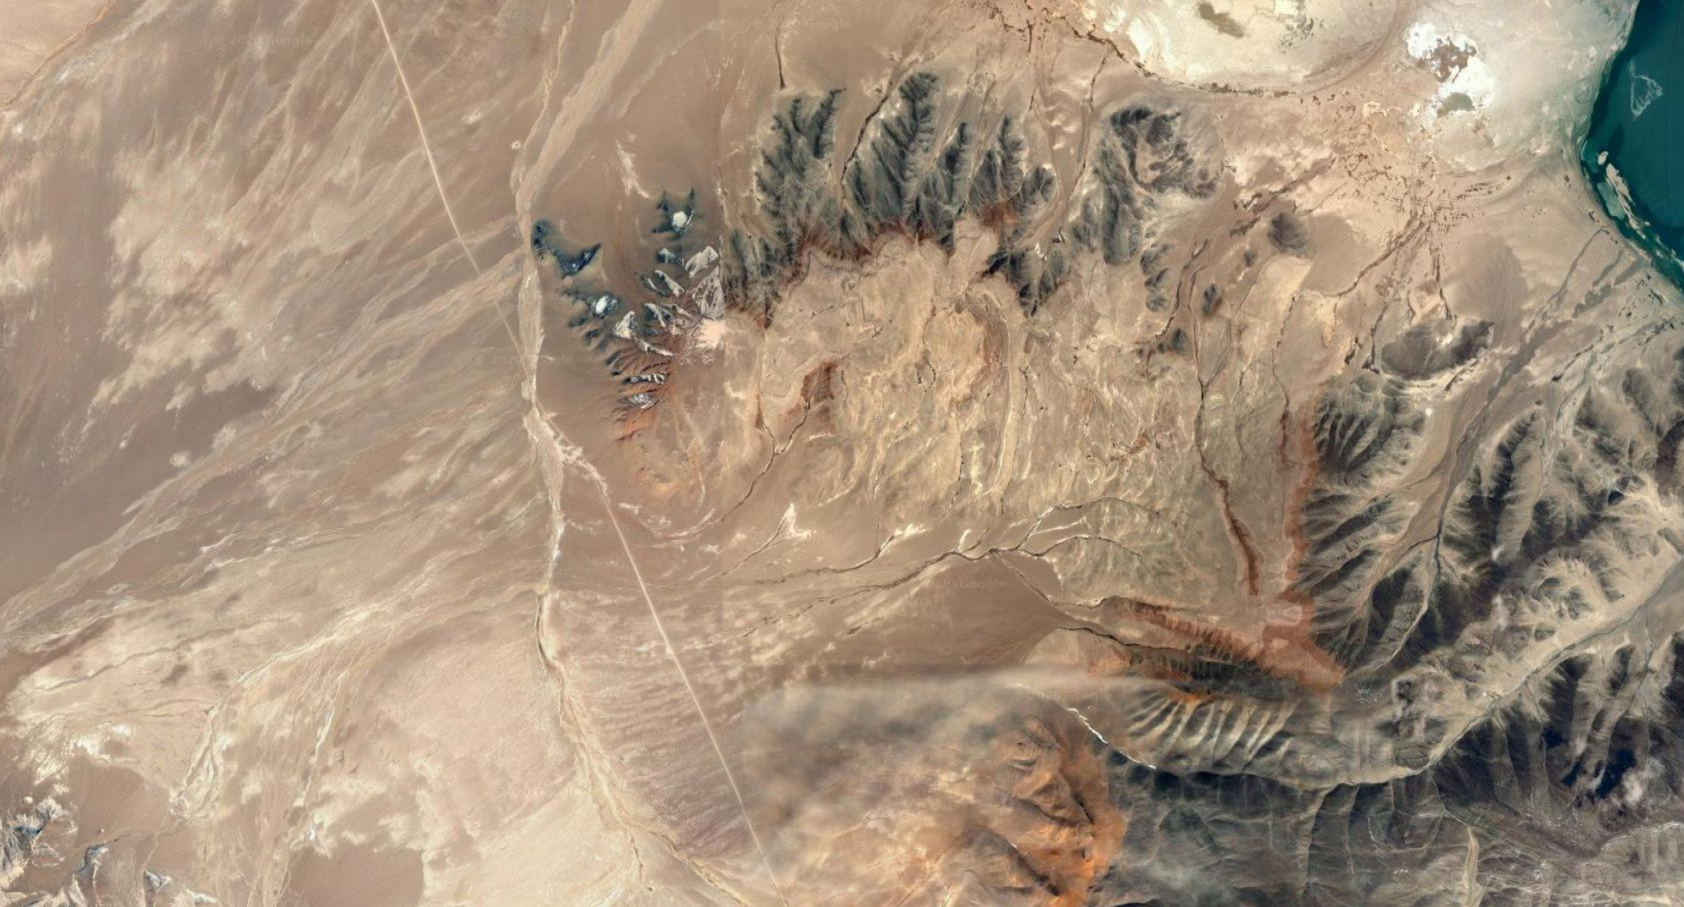
\includegraphics[width=\linewidth]{img/india_jammuAndKashmir_road.png}
	\caption{Satellite image of a part of Aksai Chin from Google Maps. The road goes from the top left to the bottom centre of the image and has a light brown colour.}
	\label{pic:india_jammuAndKashmir_road}
	\end{figure}
	
	\subsection{Arunachal Pradesh}
	Arunachal Pradesh is a region located between China and India both regionally and culturally. While it is governed by India the native spoken language in this region is Tibetan. Therefore, China claims the region it refers to as South Tibet.
	
	\subsection{Nepal}
	A natural border is formed between Nepal and China: the Himalayas. The highest peak, Mount Everest, can be reached from both sides and lies exactly on the border.
	
	\section{Hong Kong and Macau}
	The border between Hong Kong and China divides not countries, but values. Both Hong Kong and Macau were foreign colonies and are therefore what is called a special administrative region, which means they can have their own laws.
	
	One of the most obvious differences between mainland China and Macau it the absence of the law that forbids gambling. This has transformed Macau's skyline into string of casinos. In 2018 the World Bank estimated Macau's GDP to be around 54 billion US dollars.
	
	Hong Kong on the other hand is known for its freedom of speech, which has led many people reporting on the Chinese regime to move to this island. China, however, is starting to intervene in the high valued right of freedom. The protest from the Hong Kong citizens against this behavior was called umbrella movement.
	
	Both borders are separating China from what is technically also China. The procedure of crossing is very similar to an international border, as you need your passport and a visa for China\cite{macauLifestyle_macauZhuhaiTheUltimateBorderCrossingGuide} \cite{yp_chinaIsErasingItsBorderWithHongKong}.
	
	\section{South China Sea}
	The Spratly Islands, located in the South China Sea, near the shore of the Philippines, are the objective of a relatively new extension of Chinas borders. Since 2014 seven of the reefs located there have had huge amounts of sand heaped on them. Now the newly formed islands serve military purposes, as can be seen in figure~\ref{pic:southChinaSea_subiReef}. By owning these islands China would increase exclusive economic zone, defined by the United Nations Convention on the Law of the Sea\cite{unitedNations_lawOfTheSea}.
	
	\begin{figure}[t]
		\centering
		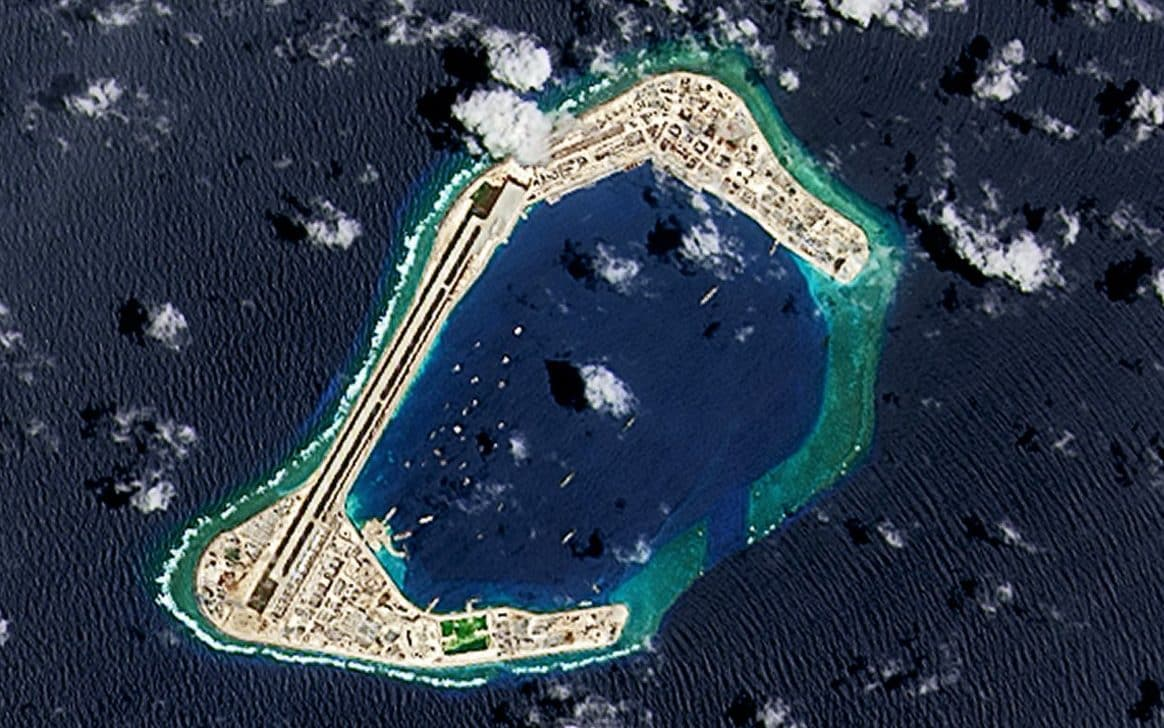
\includegraphics[width=\linewidth]{img/southChinaSea_subiReef.jpg}
		\caption{Satellite image of Subi Reef\cite{theTelegraph_chinaLandsMilitaryPlaneAtThirdSpratlyIsland}. The runway and some boats are clearly visible.}
		\label{pic:southChinaSea_subiReef}
	\end{figure}
	
	\section{Mongolia}
	Next to Mongolia lies the Chinese province of Inner Mongolia. In this province the Great Wall of China protected Chinese citizens from Mongols in the \nth{5} century BC up until the \nth{17} century AD\cite{worldAtlas_whyWasTheGreatWallOfChinaBuilt}. As the map of the Great Wall of China shows, rather than building a single line where the border is, the wall was constructed over a long period of time and moved regularly. This can be seen in figure~\ref{pic:mongolia_greatWallOfChina}.
	
	\begin{figure}[t]
		\centering
		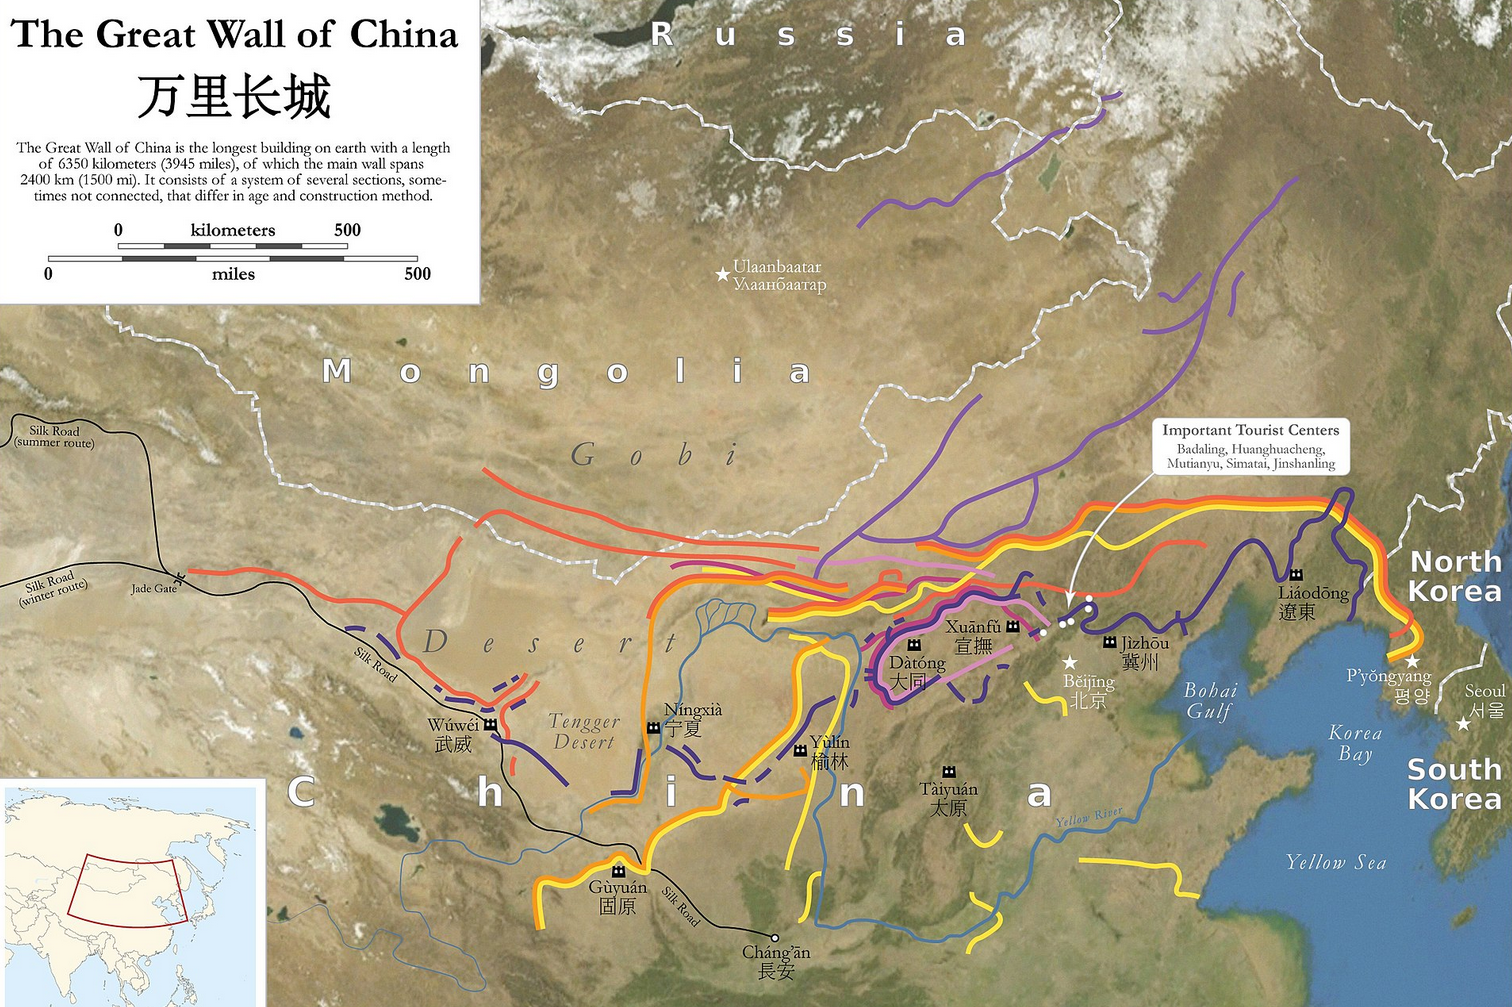
\includegraphics[width=\linewidth]{img/mongolia_greatWallOfChina.png}
		\caption{A section of the map published by Wikipedia\cite{wp_greatWallOfChina}. The different colours represent different ages in which the sections where constructed. The light purple lines represent wall segments from the \nth{11} and \nth{12} century AD and extend north into nowadays Mongolia and Russia.}
		\label{pic:mongolia_greatWallOfChina}
	\end{figure}

	Since then the Mongol Empire has collapsed. Now most people with a Mongol ethnicity live in Inner Mongolia (about 50\% more than in the state Mongolia).
	
	The Trans-Siberian Railway, partly running through Mongolia, transports travelers and freight between Russia and China. Now this railway network is becoming part of Chinas Belt and Road Initiative.
	
	\section{Myanmar}
	Its geographic location made Chinas Petroleum and Chemical Corporation interested in Myanmar. Before 2014 most of Chinas oil and natural gas imports were shipped from Africa and the Middle East over the Indian Ocean and through the Malacca Strait before arriving at a Chinese port. With the building of a pipeline, connecting the deep-water port of Kyaukphyu to the Yunnan province in China, a new route was secured\cite{chinaDaily_oilStartsFlowingThroughChinaMyanmarPipeline}.
	
	The construction work of the pipeline and the deep-water port were partly done by Chinese workmen, while many of the simple tasks were given to local people. Additionally, China tries to get more popular with the Myanmar population by financing schools and opening the border. These influences have persuaded many parents to get their children to learn Mandarin. They believe that it will be easier to get jobs when being able to communicate with Chinese\cite{yt_oneVillageTwoCountriesNoBorderTheNewSilkRoadCNAInsider}.
	
	\section{Laos and Vietnam}
	The Laos-China and Vietnam-China border are characterized by huge rainforest areas. Only few cities are located near the border.
	
	Historically China disliked Vietnam and Laos, even though they are communist lead states, because they did not want to follow Maoism, Chinas idea of how a communist state should be run.
	
	\subsection{Laos}
	Laos shares two border crossings with China, only one of which can be accessed by third-country citizens. The rest of the border is lined with rainforest sometimes interrupted by coffee plantations.
	
	\subsection{Vietnam}
	A railway connects Nanning in China to Hanoi in Vietnam. It allows travelers to make the journey by night in one of the night trains available.
	
	Once arriving at the border however, the passengers are awoken by Chinese border guards collecting all passports and requesting all passengers to collect their belongings and leave the train. While the train is inspected other Chinese staff sort through all passports. After everything has been checked the train can be boarded again and the passports are handed back.
	
	After having travelled a few hundred meters the guests are once again requested to leave the train and hand over their passports, this time to the Vietnamese border patrol. Passports are checked once again and then slowly handed back by a soldier trying to read the names out to the group of waiting tourists. Back inside the train the journey is continued, without any further stop until reaching the destination.
	
	\section{Bhutan}
	During an uprising in Tibet the spiritual leader, Dalai Lama, fled to India\cite{time_howAndWhyTheDalaiLamaLeftTibet}. Following him, many Buddhists from Tibet sought asylum in Bhutan, even though the border is formed by high mountain chains of the east Himalayas. The fear of more refugees led to the enforcement of protection along the border to China.
	
	\section{Russia}
	Chinas largest neighbor, Russia, was hugely influential for Chinese politics. After communism started there, it spread to China where Mao Zedong rose to power. After Stalin's death his successor, Khrushchev, criticized some of Stalin's steps. Mao feared that he would face the same future. He decided that the way to not be forgotten by history would be by splitting Chinas views on communism from Russia.
	
	This led to tensions in the relations between China and Russia. Over multiple years two border disputes occurred. These have been settled since.
	
	The border to Russia consists of a short west section and the longer east section, where all border crossings are located. By travelling with the Trans-Siberian Railway one can reach the north east of China from Moscow.
	
	\section{Kazakhstan, Kyrgyzstan and Tajikistan}
	The borders between China and the three countries Kazakhstan, Kyrgyzstan and Tajikistan were largely defined by the territory owned by Russia before its collapse.
	
	Now some border crossings connect to China by road and two railway border crossings in Kazakhstan make travel to China by train possible.
	
	\subsection{Belt and Road Initiative}
	Kazakhstan lies between China and Moscow from where Europe can easily be reached by the existing railway network. So, it's no wonder Kazakhstan invested 30 billion US dollars to building infrastructure connecting China to the west. It can be estimated that the annual income from transport fees totals up to nearly 5 billion US dollars.
	
	Other countries in the region are following Kazakhstan's plan with China being ready to invest.
	
	\section{Afghanistan}
	The thin Wakhan Corridor (part of Afghanistan) connects the country to China. The corridor was used by merchants travelling along the Silk Road to reach China. Nowadays the border crossing marks a jump in time zones of 3\sfrac{1}{2} hours and is closed.
	
	\section{Conclusion}
	This topic gives an insight in the history of most Asian countries spanning the last few centuries. It shows the transformation of land where once no borders existed to the lines existing today. Chinas position in the world is emphasized by its longing for more influence. Trading, which had a big impact on China in the past, is nowadays living up even more than expected. However, all borders are currently closed and the future for many of them seem unclear, as the pandemic of covid-19 is stopping global travel.
	
	\section*{Acknowledgment}
	The author would like to thank Johnny Harris for producing the interesting border series and family and friends for specifying the topic and suggesting China as the focus point.
	
	\bibliographystyle{plain}
	\bibliography{main}
\end{document}


